%\section{Tensor Factorization}  \label{sec:tf}

\section{Multivariate Factorization Model} \label{sec:tf}
A given sensor node may contain multiple sensor types and thus able to sense various aspects of its environment (e.g.\ temperature and humidity) at the same time.
These attributes may be correlated and this correlation may help in the missing data estimation process.
We propose two methods, Multivariate (S)TR-MF and Tensor Factorization, that leverage this multivariate correlation.

\subsection{Multivariate (S)TR-MF} %\label{subsec:Multivariate_TRMF}
If two matrices are correlated, then some of their latent factors should be similar.
This motivates us to design Multivariate (S)TR-MF.

Assume we have two attributes: temperature and humidity.
The $\mathbf{R}$ of Multivariate (S)TR-MF is the horizontal concatenation of the temperature matrix $\mathbf{R}_{tem}$ and $\mathbf{R}_{hum}$
\begin{equation*} \mathbf{R} = \begin{bmatrix}\mathbf{R}_{tem} & \mathbf{R}_{hum} \end{bmatrix} \end{equation*}

The objective function is similar to (S)TR-MF except that for each row (time step) there are two bias terms: one for temperature readings and the other for humidity readings.
Now $\mathbf{R}_{tem}$ and $\mathbf{R}_{hum}$ of $\mathbf{R}$ must be normalized independently with their own means and variances.
The optimization process remains the same as in Section \ref{optimation_procedure}.

Factorization models for tensors have been studied for many years~\cite{tg2009td}~\cite{bergqvist2010hosvd}. The main idea behind the use of Tensor Factorization (TF) is that we can take advantage of the principle behind Matrix Factorization to deal with additional features of the dataset. In sensor network data, temporal, spatial, and heterogeneous sensor information can be strongly correlated.
Modeling these correlation can thus be a great benefit when estimating missing values.
 
Tensor decomposition is a multi-dimensional extension of Singular Value Decomposition (SVD).
In the section \ref{sec:sensordecomp} we introduce the methods of Tensor Decomposition.
A general model of tensor decomposition is the Tucker decomposition (TD) also known as High-Order Singular Value Decomposition (HOSVD).
The special case of Tucker decomposition is called canonical decomposition (CD) also known as parallel factor analysis (PARAFAC).
Tensor Decomposition methods require a dense input matrix $\mathbf{R}$ with missing parts of input data ignored during optimization.
%Treating $\mathbf{R}$ as a dense tensor with missing entries being assume to be 0.
%It would make predict missing value failed.
We introduce and explain the details of how we have adapted the Tensor Decomposition models with latent factors for missing value estimation in Section \ref{sec:tfmissing}.
 
\subsection{Tensor Decomposition} \label{sec:tensordecomp}

 If we want to decompose a $m\times n$ Matrix M, recall the Singular Value Decomposition(SVD) as being
\begin{equation*} 
\mathbf{M}=\mathbf{P}\Sigma \mathbf{Q}^\mathrm{T}=\sum\limits_{k=1}^r\sigma_kp_kq_k^\mathrm{T}=\sum\limits_{k=1}^r\sigma_kp_k\otimes q_k
\end{equation*}
Where $\otimes$ denoted the tensor product : $x\otimes y = xy^\mathrm{T}$.
$r$ is the rank of $\mathbf{M}$,
$\mathbf{P}$ is an $m\times m$ unitary matrix, $\mathbf{Q}$ is a $n\times n$ unitary matrix, $\Sigma$ is an $m\times n$ rectangular diagonal matrix with singular values of M, being adopted the following convention $\sigma_1>\sigma_2 >...\sigma_r>0=\sigma_{r+1}=...=\sigma_{n}$.
The SVD may be generalized to High-Order Tensor decomposition.
the following are two types of tensor decomposition, for simplicity and in practical, we present the decomposition for 3-order tensor.

\subsubsection{Tucker Decomposition}
The Tucker decomposition was first introduced by Tucker in 1963 [1], it factorizes a higher-order tensor into a core tensor $\mathbf{S}$ and a factor matrix for each dimensions.
We decompose a $M\times N \times C $ tensor $\mathbf{T}$ :

\begin{equation*}
\mathbf{T}=\sum\limits_{i=1}^{I}\sum\limits_{j=1}^{J}\sum\limits_{k=1}^{K}\mathbf{S}_{ijk}p_i\otimes q_j\otimes w_k
\end{equation*}
or for each component,
\begin{equation*}
\mathbf{T}_{mnc}=\sum\limits_{i=1}^{I}\sum\limits_{j=1}^{J}\sum\limits_{k=1}^{K}\mathbf{S}_{ijk}\mathbf{P}_{m i}\mathbf{Q}_{n j}\mathbf{W}_{c k}
\end{equation*}
where the vectors $p_i$, $q_j$, and $w_k$ are the column of matrices $\mathbf{P}$, $\mathbf{Q}$ and $\mathbf{W}$ respectively, which are the factor matrices and usually orthogonal.
They can be thought of as the principal components in each order.
There are several algorithms for calculating Tucker decompositions.
For data compression, the Tucker decomposition usually assumes that $I\le M$, $J \le N $ and $K \le C$.

\subsubsection{Canonical Decomposition}

The Canonical decomposition factorizes a tensor into a sum of component rank-one tensors.
Formally, the Canonical Decomposition(CD) is the special case of the Tucker decomposition when $\mathbf{S}$ is superdiagonal.
The Canonical Decomposition of $\mathbf{T}$ is
\begin{equation*}
\mathbf{T}=\sum\limits_{k=1}^{K}x_k\otimes y_k\otimes z_k
\end{equation*}
or
\begin{equation*}
\mathbf{T}_{mnc}=\sum\limits_{k=1}^{K}\mathbf{X}_{m k} \mathbf{Y}_{n k} \mathbf{Z}_{c k}
\end{equation*}
where $x_i$,$y_i$ and $z_i$ are the column of matrices $\mathbf{X}$, $\mathbf{Y}$ and $\mathbf{Z}$, which are the factor matrices, $K$ is the factor size. 

The Tucker Decomposition and Canonical Decomposition are illustrated in Figure \ref{fig:tf:tuckcanon}.

\begin{figure}[h] 
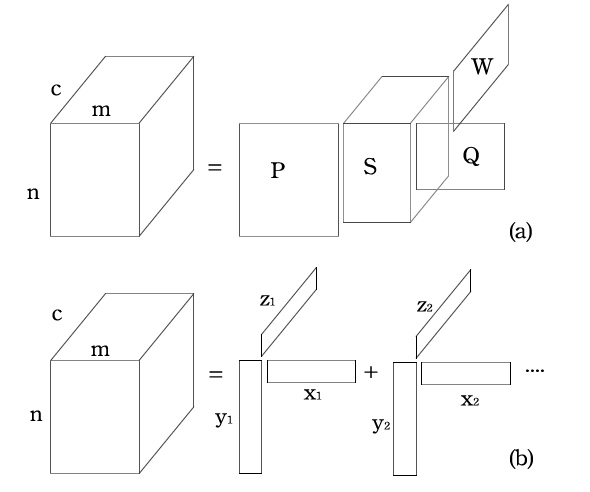
\includegraphics[width=9cm]{tf.jpg} 
\caption{ (a) the Tucker Decomposition (TD) model (b) the Canonical Decomposition model, a special case of the TD model.In sensor networks, the three dimension can be nominal features such as node id, time step index.} 
\label{fig:tf:tuckcanon} 
\end{figure}

\subsection{Tensor Factorization for Missing Data Estimation} \label{sec:tfmissing}
\subsubsection{Objective function}

Existing Tensor Decomposition models require a dense tensor, which is unsuitable for missing data estimation with a high missing rate. 
Therefore, we introduce an $N$-order Tensor Factorization for missing data estimation. In the CF technology, the TF also use in context-aware recommender system recently~\cite{karatzoglou2010multiverse}~\cite{steffen2010pairwise}~\cite{zeno2010context}.
Just like MF, it takes advantage of data sparsity while still exploiting the temporal correlation.
Moreover, it models the correlation between different information, e.g.\ spatial correlation and heterogeneous sensor readings.
The followings are the details of the model we propose.

Assume that there are three features $F_1, F_2 , F_3$, $F_1$ is the time step number, $F_2$ and $F_3$ are the other features, it could be the sensor node ID, sensor node coordinates, heterogeneous sensor readings or other information.
suppose the target sensor readings is $R$ such that tensor T containing  $R$ will be 3-dimensional tensor :
\begin{equation*}
\mathbf{T} := \mathbf{F_1} \times  \mathbf{F_2} \times \mathbf{F_3} \rightarrow \mathbf{R}
\end{equation*}

In contrast to conventional tensor decomposition, the learning model we propose is learning the latent factors $\mathbf{P}$,  $\mathbf{Q}$, $\mathbf{W}$.
Where $\mathbf{P}$,  $\mathbf{Q}$, $\mathbf{W}$ are the factors of $F_1, F_2, F_3$.
To avoid over-fitting and decrease the complexity of computing prediction, our model is based on Canonical Decomposition.
Its complexity of computing prediction is $\mathbf{O}(K)$, where K is the factor size of  P, Q and W.
On the other hand, the complexity of Tuker Decomposition is $\mathbf{O}(K^3)$  by our optimization method,
where $ K=min(K_P,K_Q,K_W) $ , $K_P$, $K_Q$, $ K_W$ are the factor size of $\mathbf{P}$,  $\mathbf{Q}$, $\mathbf{W}$ respectively.

As MF, to increase the prediction accuracy, we also add bias term of $F_1, F_2, F_3$ into our Tensor Factorization model.
so our prediction function is :
\begin{equation*}
\begin{aligned}
\mathbf{\hat{T}}_{mnc}=\mu_m+\mu_n+\mu_c+p_m \otimes q_n\otimes  w_c
\\=\mu_m+\mu_n+\mu_c+\sum\limits_{k=1}^{K}\mathbf{P}_{m k} \mathbf{Q}_{n k} \mathbf{W}_{c k}
\end{aligned}
\end{equation*}
to learn the latent features P, Q and W, we define the loss function :
\begin{equation*}
L(\mathbf{\hat{T}},\mathbf{T})=\frac{1}{\|\mathbf{D}\|_1} \sum\limits_{t\in \mathbf{D}}  l(\hat{t},t)
\end{equation*}
where $\mathbf{D}$ is the dataset and $\|\mathbf{D}\|$ means the amounts of data point.
$l$ is a point-wise loss function penalizing the distance between estimate and observation.
we choose $l$ being least squared error because the evaluation function is root mean square error (RMSE), so
\begin{equation*}
l(\hat{t},t)=\frac{1}{2}(t-\hat{t})^2
\end{equation*}

Simply minimizing a loss function is known to lead to over-fitting.
Given the factors P, Q, W and bias terms which constitute our model, we have a choice of ways to ensure that the model complexity does not grow without bound.
we add a regularization term based on the $l_2$ norm of these
factors.
To capture the temporal effect, similar to MF we state previous in section 3.2, we add the time regularization term to our model.
Finally, the objective function of tensor factorization is :\\
\begin{equation*}
\begin{aligned}
&\sum\limits_{m, n, c} l( \hat{\mathbf{T}}_{mnc}, \mathbf{T}_{mnc} )+\beta_1\|p_{\beta}\|^2+\beta_2\|q_n\|^2+\beta_3\|w_c\|^2+\beta_4\|
\mu_m\|^2\\
&+\beta_5\|\mu_n\|^2+\beta_6\|\mu_c\|^2+\frac{1}{2}\gamma_1\sum(\mu_m-\mu_{m+1})^2+(\mu_m-\mu_{m-1})^2
\\&
+\frac{1}{2}\gamma_2\sum(p_m-p_{m+1})^2+(p_m-p_{m-1})^2
\end{aligned}
\end{equation*}

\begin{algorithm}[h]
  \caption{Multivariate Tensor Factorization}
  \label{alg::conjugateGradient}
  \begin{algorithmic}[1]
    \Require
    $\beta_1,\beta_2, \beta_3, \beta_4, \beta_5, \beta_6, \gamma_1, \gamma_2, \eta, k$
    \State Normalize the training set as $D$
    \State initial the $p_m, q_n, w_c, \mu_m, \mu_n, \mu_c$ for all $m, n, c$
    \Repeat
      \For    {each observed readings t in D}
      \State Update $p_m, q_n, w_c, \mu_m, \mu_n, \mu_c$ 
     \EndFor
     \State Update $p_m,  \mu_m $ for all m
    \Until stopping criterion is met
    \State Output the model 
  \end{algorithmic}
\end{algorithm}

\subsubsection{Optimization}
Minimizing this objective function can be done using many approaches.
To deal with large datasets, there are simple and fast online algorithm which performs stochastic gradient descent (SGD) in the factors for a given tuple t simultaneously.
we need to compute the gradients of the objective function with respect individual components of the model.
Focus on a observed data t = $T_{m\beta\gamma } $ from training data, the update rule is :
\begin{equation*}
\begin{aligned}
&{p_m}^\prime={p_m}+\eta(e*q_n w_c - \beta_1 p_m)
\\&{q_n}^\prime={q_n}+\eta(e*p_m w_c - \beta_2 q_n)
\\&{w_c}^\prime={w_c}+\eta(e*p_m q_n - \beta_3 w_c)
\\&{\mu_m}^\prime=\mu_m+\eta(e-\beta_4\mu_m)
\\&{\mu_n}^\prime=\mu_n+\eta(e-\beta_5\mu_n)
\\&{\mu_c}^\prime=\mu_c+\eta(e-\beta_6\mu_c)
\end{aligned}
\end{equation*}
where $e=t-\hat{t}$, After a iteration, we update the model according to the temporal regularization :
\begin{equation*}
\begin{aligned}
&{p_m}^\prime={p_m}+\eta\gamma_1(p_{m+1}-p_m+p_{m-1}-p_m)
\\&{\mu_m}^\prime=\mu_m+\eta\gamma_2(\mu_{m+1}-\mu_m+\mu_{m-1}-\mu_m)
\end{aligned}
\end{equation*}
The Tensor Factorization method is summarized in Procedure 2, which is easy to implement since it accesses only one row of P, Q ,W at a time.

The details about normalization, initialization and stop criterion are just like MF, which are stated in previous part.
The parameters of TF are more than MF, but we can achieve reasonable performance by setting
\begin{equation*}
\begin{aligned}
& \beta_1=\beta_2=\beta_3=\beta_4=\beta_5=\beta_6\\
&\gamma_1=\gamma_2\\
\end{aligned}
\end{equation*}
